\chapter{Curvature from Commutators and the Newtonian Limit}

Curvature is easy to picture and harder to calculate. A vector carried
around a small closed loop generally returns with a changed orientation,
but turning that geometric statement into a usable formula requires
careful notation. We shall introduce only as much operator language as is
needed to make the calculation transparent. The reward is substantial:
the Riemann tensor will emerge as a commutator, its contractions will lead
to the Ricci tensor and scalar curvature, and the same geometric language
will then meet Newtonian gravity in the weak-field limit.

The lecture has two distinct movements. The first is mathematical. We
derive curvature by comparing covariant differentiation in two orders.
The second is physical. We place a slowly moving particle in a weak,
nearly static field and ask how the geodesic equation can reproduce
\(F=ma\) and Poisson's equation. Those two movements meet in the search
for a generally covariant field equation.

\section{Vector Fields and Linear Operators}

Let
\begin{equation}
  V^\alpha(x)
  =
  \bigl(V^0(x),V^1(x),V^2(x),V^3(x)\bigr)
  \label{eq:l08-vector-field}
\end{equation}
be a vector field on four-dimensional spacetime. It is useful to regard
its four components as four functions collected into one column vector.
Several familiar operations on this collection are linear operators.

First, differentiation with respect to a coordinate is an operator:
\begin{equation}
  \partial_\mu V^\alpha(x)
  =
  \frac{\partial V^\alpha(x)}{\partial x^\mu}.
  \label{eq:l08-partial-operator}
\end{equation}
Second, multiplication by an ordinary function is an operator:
\begin{equation}
  F(x)\,V^\alpha(x).
  \label{eq:l08-function-operator}
\end{equation}
Third, a matrix acts on the component index:
\begin{equation}
  (MV)^\alpha=M^\alpha{}_\beta V^\beta.
  \label{eq:l08-matrix-operator}
\end{equation}
The matrix may itself depend on position,
\(M^\alpha{}_\beta=M^\alpha{}_\beta(x)\). These examples are not an
exhaustive catalogue; they are exactly the ingredients needed below.

\begin{figure}[tbp]
  \centering
  
\includegraphics[width=0.84\textwidth]{lecture_08_figure_01.png}
  \caption{Derivative, function-multiplication, and matrix-multiplication
  operators acting on the component functions of a vector field. The
  final line allows the matrix itself to depend on position.}
  \lectureframe{00:07:45}
\end{figure}

The covariant derivative combines differentiation with a
position-dependent matrix:
\begin{equation}
  (\nabla_\mu V)^\alpha
  =
  \partial_\mu V^\alpha
  +
  \Gamma^\alpha{}_{\mu\beta}V^\beta.
  \label{eq:l08-covariant-derivative}
\end{equation}
For each fixed value of \(\mu\), define the matrix
\begin{equation}
  (\Gamma_\mu)^\alpha{}_\beta
  =
  \Gamma^\alpha{}_{\mu\beta}.
  \label{eq:l08-connection-matrix}
\end{equation}
Then the same definition can be written schematically as
\begin{equation}
  \boxed{\nabla_\mu=\partial_\mu+\Gamma_\mu.}
  \label{eq:l08-operator-covariant-derivative}
\end{equation}
The indices \(\alpha,\beta\) are hidden matrix indices; \(\mu\) labels
which directional derivative and which connection matrix are being used.
Whenever the compact notation becomes ambiguous, Eq.~\eqref{eq:l08-covariant-derivative}
restores all three roles.

\begin{figure}[tbp]
  \centering
  
\includegraphics[width=0.88\textwidth]{lecture_08_figure_02.png}
  \caption{The component definition of the covariant derivative and its
  compact operator form. The colored indices on the board distinguish
  the matrix slots from the derivative direction.}
  \lectureframe{00:12:15}
\end{figure}

\begin{classroomqa}
\audiencequestion{Why are there four connection matrices? Is that tied
to the three spatial coordinates and one time coordinate?
\lecturetimestamp{00:12:40--00:13:08}}
\lecturerresponse{Yes, in this discussion spacetime is four-dimensional,
so \(\mu\) takes four values and labels four matrices
\(\Gamma_\mu\). In an \(n\)-dimensional manifold there would be \(n\)
such matrices, each of size \(n\times n\). The construction is not tied
to four dimensions.}
\end{classroomqa}

\section{The One Commutator Identity We Need}

For two operators \(A\) and \(B\), their product \(AB\) means that \(B\)
acts first and \(A\) acts second. Their commutator is
\begin{equation}
  [A,B]=AB-BA.
  \label{eq:l08-commutator}
\end{equation}
For noncommuting operators, reversing the sequence can change the result.

Regard \(F(x)\) as the operator that multiplies by the function \(F\).
The elementary identity needed for curvature is
\begin{equation}
  \boxed{[\partial_x,F(x)]=\frac{dF}{dx}.}
  \label{eq:l08-derivative-function-commutator}
\end{equation}
This is an operator identity, so its meaning must be tested on an
arbitrary function \(V(x)\):
\begin{align}
  [\partial_x,F]V
  &=
  \partial_x(FV)-F\partial_xV
  \notag\\
  &=
  \frac{dF}{dx}V
  +
  F\frac{dV}{dx}
  -
  F\frac{dV}{dx}
  \notag\\
  &=
  \frac{dF}{dx}V.
  \label{eq:l08-commutator-proof}
\end{align}
The terms in which the derivative acts on \(V\) cancel. The remaining
instruction is simply multiplication by \(dF/dx\).

\begin{figure}[tbp]
  \centering
  
\includegraphics[width=0.84\textwidth]{lecture_08_figure_03.png}
  \caption{The compact covariant-derivative notation, the definition of
  a commutator, and the derivative--multiplication identity that drives
  the curvature calculation.}
  \lectureframe{00:15:30}
\end{figure}

\begin{figure}[tbp]
  \centering
  
\includegraphics[width=0.82\textwidth]{lecture_08_figure_04.png}
  \caption{The product-rule calculation behind
  Eq.~\eqref{eq:l08-derivative-function-commutator}. The two terms in
  which the derivative reaches the test function cancel.}
  \lectureframe{00:18:30}
\end{figure}

The same identity holds component by component when \(F\) is replaced by
a matrix-valued function such as \(\Gamma_\mu(x)\):
\begin{equation}
  [\partial_\nu,\Gamma_\mu]
  =
  \partial_\nu\Gamma_\mu.
  \label{eq:l08-matrix-commutator-lemma}
\end{equation}
This does not mean that a matrix has become a scalar. It means that every
matrix entry is differentiated.

\section{A Loop as a Difference of Differences}

Choose two infinitesimal displacement vectors,
\(\epsilon^\mu\) and \(\eta^\nu\), spanning a small parallelogram. Label
its corners \(A,B,C,D\), and parallel transport a vector successively
along
\[
  A\longrightarrow B\longrightarrow C\longrightarrow D
  \longrightarrow A.
\]
The base point returns to \(A\), but the transported vector need not
return with the same components. Denote the initial vector by \(V_A\)
and the final one by \(V_A'\).

\begin{figure}[tbp]
  \centering
  
\includegraphics[width=0.84\textwidth]{lecture_08_figure_05.png}
  \caption{The transported vector around an infinitesimal loop. The
  dashed offset at \(A\) records its change in orientation after the
  path has returned to its starting point.}
  \lectureframe{00:23:30}
\end{figure}

\begin{classroomqa}
\audiencequestion{Does the vector fail to return to the same point, or
does it return to the point with a different orientation?
\lecturetimestamp{00:24:03--00:24:15}}
\lecturerresponse{The path closes at the same point. It is the
transported vector that returns changed. The small separation drawn
between \(V_A\) and \(V_A'\) is a picture of that change in the vector
space at \(A\).}
\end{classroomqa}

The loop mismatch can be isolated by an intentionally engineered
difference of differences:
\begin{align}
  &\bigl[(V_C-V_D)-(V_B-V_A)\bigr]
  \notag\\
  &\qquad
  -
  \bigl[(V_C-V_B)-(V_D-V_A')\bigr]
  =
  V_A-V_A'.
  \label{eq:l08-finite-difference-identity}
\end{align}
Every intermediate value cancels. The first bracket compares horizontal
differences after a vertical displacement; the second compares vertical
differences after a horizontal displacement. In the infinitesimal limit
these become two second-order operations taken in opposite orders.

\begin{figure}[tbp]
  \centering
  
\includegraphics[width=0.88\textwidth]{lecture_08_figure_06.png}
  \caption{The board construction of the two finite differences. The
  circled terms cancel, leaving only the initial--final mismatch.}
  \lectureframe{00:30:15}
\end{figure}

\begin{classroomqa}
\audiencequestion{Why subtract the two differences in this order rather
than the reverse order?
\lecturetimestamp{00:27:41--00:29:05}}
\lecturerresponse{The order fixes an orientation and is chosen so the
intermediate vectors cancel. Reversing the order reverses the sign of
the answer. Nothing physical depends on that choice once the loop
orientation and the commutator convention are stated consistently.}
\end{classroomqa}

Because the vectors at neighboring points must be compared by parallel
transport, ordinary derivatives are not adequate. The finite
differences become covariant derivatives. With the convention
\begin{equation}
  [\nabla_\mu,\nabla_\nu]V^\alpha
  =
  R^\alpha{}_{\beta\mu\nu}V^\beta,
  \label{eq:l08-riemann-convention}
\end{equation}
the leading holonomy around the oriented loop is
\begin{equation}
  \Delta V^\alpha
  =
  R^\alpha{}_{\beta\mu\nu}
  V^\beta\epsilon^\mu\eta^\nu
  +
  O(\ell^3),
  \label{eq:l08-loop-holonomy}
\end{equation}
where \(\Delta V^\alpha=V_A'{}^\alpha-V_A^\alpha\) for the corresponding
orientation. The characteristic edge length is \(\ell\), so the leading
change is of order \(\ell^2\).

Only the antisymmetric part of the edge product contributes. Defining
the oriented area bivector
\begin{equation}
  \Sigma^{\mu\nu}
  =
  \epsilon^\mu\eta^\nu-\epsilon^\nu\eta^\mu,
  \label{eq:l08-area-bivector}
\end{equation}
we may equivalently write
\begin{equation}
  \Delta V^\alpha
  =
  \frac12
  R^\alpha{}_{\beta\mu\nu}
  V^\beta\Sigma^{\mu\nu}
  +
  O(\ell^3).
  \label{eq:l08-holonomy-area}
\end{equation}

\begin{figure}[tbp]
  \centering
  
\includegraphics[width=0.88\textwidth]{lecture_08_figure_07.png}
  \caption{The difference of covariant differences compressed into a
  commutator. The two edge vectors supply the oriented area, and the
  commutator acts on the transported vector.}
  \lectureframe{00:36:45}
\end{figure}

\begin{classroomqa}
\audiencequestion{As the two edge vectors go to zero, what else goes to
zero? The Riemann tensor itself has no loop size in it.
\lecturetimestamp{00:50:50--00:52:24}}
\lecturerresponse{The vector change goes to zero. Curvature is the local
coefficient of that change per oriented area. Thus
\(\Delta V=O(\ell^2)\), while the Riemann tensor approaches a finite
value at the base point. A finite loop can be understood, with suitable
path ordering, as accumulated infinitesimal holonomy.}
\end{classroomqa}

\begin{classroomqa}
\audiencequestion{Should we divide the long equation by the two edge
lengths and call the result a mixed second derivative?
\lecturetimestamp{00:58:23--00:58:39}}
\lecturerresponse{Dividing by area does isolate the curvature
coefficient, but the geometric operation is not the mixed derivative of
one scalar function. It is the noncommutativity of two covariant
derivatives acting on a vector.}
\end{classroomqa}

\section{Expanding the Covariant-Derivative Commutator}

Insert Eq.~\eqref{eq:l08-operator-covariant-derivative} into the
commutator:
\begin{align}
  [\nabla_\mu,\nabla_\nu]
  &=
  [\partial_\mu+\Gamma_\mu,
    \partial_\nu+\Gamma_\nu]
  \notag\\
  &=
  [\partial_\mu,\partial_\nu]
  +
  [\partial_\mu,\Gamma_\nu]
  -
  [\partial_\nu,\Gamma_\mu]
  +
  [\Gamma_\mu,\Gamma_\nu].
  \label{eq:l08-expanded-commutator}
\end{align}
For smooth fields in a coordinate basis,
\begin{equation}
  [\partial_\mu,\partial_\nu]=0.
  \label{eq:l08-partials-commute}
\end{equation}
The mixed terms are evaluated with
Eq.~\eqref{eq:l08-matrix-commutator-lemma}, while the last term remains
because matrix multiplication is generally noncommutative:
\begin{equation}
  [\nabla_\mu,\nabla_\nu]
  =
  \partial_\mu\Gamma_\nu
  -
  \partial_\nu\Gamma_\mu
  +
  \Gamma_\mu\Gamma_\nu
  -
  \Gamma_\nu\Gamma_\mu.
  \label{eq:l08-curvature-matrix}
\end{equation}

\begin{figure}[tbp]
  \centering
  
\includegraphics[width=0.9\textwidth]{lecture_08_figure_08.png}
  \caption{The operator expansion on the board. Ordinary derivative
  terms cancel, derivative--connection commutators produce
  \(\partial\Gamma\), and the connection matrices leave a genuine
  matrix commutator.}
  \lectureframe{00:42:45}
\end{figure}

\begin{classroomqa}
\audiencequestion{What is the derivative of \(\Gamma_\nu\) if
\(\Gamma_\nu\) is a matrix?
\lecturetimestamp{00:42:54--00:43:24}}
\lecturerresponse{It is the matrix obtained by differentiating each
entry:
\[
  (\partial_\mu\Gamma_\nu)^\alpha{}_\beta
  =
  \partial_\mu
  \Gamma^\alpha{}_{\nu\beta}.
\]
The matrix indices were suppressed only to make the operator algebra
legible.}
\end{classroomqa}

Restoring those indices gives the Riemann tensor in the convention of
Eq.~\eqref{eq:l08-riemann-convention}:
\begin{equation}
  \boxed{
  \begin{aligned}
    R^\alpha{}_{\beta\mu\nu}
    &=
    \partial_\mu\Gamma^\alpha{}_{\nu\beta}
    -
    \partial_\nu\Gamma^\alpha{}_{\mu\beta}\\
    &\quad+
    \Gamma^\alpha{}_{\mu\lambda}
    \Gamma^\lambda{}_{\nu\beta}
    -
    \Gamma^\alpha{}_{\nu\lambda}
    \Gamma^\lambda{}_{\mu\beta}.
  \end{aligned}}
  \label{eq:l08-riemann-components}
\end{equation}
Changing the order in the defining commutator changes the overall sign;
changing the loop orientation does the same. The convention matters, but
no geometric conclusion depends on selecting one convention rather than
the other.

\begin{figure}[tbp]
  \centering
  
\includegraphics[width=0.94\textwidth]{lecture_08_figure_09.png}
  \caption{The completed board derivation: the connection derivatives
  and quadratic connection terms act on \(V^\beta\), and the two edge
  vectors convert the curvature operator into the loop change
  \(\Delta V^\alpha\).}
  \lectureframe{00:47:15}
\end{figure}

\begin{classroomqa}
\audiencequestion{Did choosing the two edge vectors select only one
plane? Does the curvature depend on that choice?
\lecturetimestamp{00:48:58--00:50:47}}
\lecturerresponse{The two vectors do select an infinitesimal plane, but
they do not change the tensor. They contract the same
\(R^\alpha{}_{\beta\mu\nu}\) with a different area bivector and thereby
select different components of the local curvature map.}
\end{classroomqa}

\section{Symmetries and the Content of Curvature}

Lower the first index:
\begin{equation}
  R_{\alpha\beta\mu\nu}
  =
  g_{\alpha\rho}R^\rho{}_{\beta\mu\nu}.
  \label{eq:l08-lowered-riemann}
\end{equation}
For the Levi--Civita connection, the fully lowered tensor satisfies
\begin{align}
  R_{\alpha\beta\mu\nu}
  &=-R_{\beta\alpha\mu\nu},
  &
  R_{\alpha\beta\mu\nu}
  &=-R_{\alpha\beta\nu\mu},
  \label{eq:l08-pair-antisymmetries}\\
  R_{\alpha\beta\mu\nu}
  &=R_{\mu\nu\alpha\beta},
  &
  R_{\alpha[\beta\mu\nu]}
  &=0.
  \label{eq:l08-pair-exchange-bianchi}
\end{align}
The first antisymmetry follows because parallel transport preserves inner
products when the connection is compatible with the metric. The second
follows from the commutator. The third exchanges the two antisymmetric
index pairs. The last is the algebraic, or first, Bianchi identity.

\begin{figure}[tbp]
  \centering
  
\includegraphics[width=0.9\textwidth]{lecture_08_figure_10.png}
  \caption{The Riemann formula followed by its lowered-index symmetry
  bookkeeping. The board emphasizes sign reversal within either index
  pair and equality under exchange of the two pairs.}
  \lectureframe{00:54:15}
\end{figure}

\begin{classroomqa}
\audiencequestion{Does the Riemann tensor have a cyclic or sum
property?
\lecturetimestamp{00:55:57--00:56:20}}
\lecturerresponse{Yes. In the present torsion-free geometry,
\[
  R_{\alpha\beta\mu\nu}
  +
  R_{\alpha\mu\nu\beta}
  +
  R_{\alpha\nu\beta\mu}
  =0,
\]
which is \(R_{\alpha[\beta\mu\nu]}=0\). Together with the pair
symmetries, this identity removes additional apparent components.}
\end{classroomqa}

These symmetries give
\begin{equation}
  N_R(n)=\frac{n^2(n^2-1)}{12}
  \label{eq:l08-riemann-component-count}
\end{equation}
independent components in \(n\) dimensions. Thus the exact counts are
\[
  N_R(2)=1,\qquad N_R(3)=6,\qquad N_R(4)=20.
\]
A rough count of twenty-four is voiced during the lecture; the algebraic
Bianchi identity supplies the missing reduction to twenty in four
dimensions.

The derivative structure is equally important. Since
\(\Gamma\sim g^{-1}\partial g\), Eq.~\eqref{eq:l08-riemann-components}
contains
\begin{equation}
  Riemann
  \sim
  \partial^2 g
  +
  (g^{-1}\partial g)(g^{-1}\partial g).
  \label{eq:l08-riemann-derivative-structure}
\end{equation}
Some terms contain two derivatives acting on one metric component;
others are quadratic in first derivatives. If the metric is known as a
function of position, the curvature is therefore determined, although
the component calculation can be laborious.

\section{Ricci Tensor and Scalar Curvature}

Contraction within either antisymmetric pair gives zero. For example,
\begin{equation}
  g^{\mu\nu}R_{\alpha\beta\mu\nu}=0,
  \label{eq:l08-zero-antisymmetric-contraction}
\end{equation}
because \(g^{\mu\nu}\) is symmetric and
\(R_{\alpha\beta\mu\nu}\) is antisymmetric in \(\mu,\nu\). The same
argument applies to contraction of \(\alpha,\beta\).

\begin{figure}[tbp]
  \centering
  
\includegraphics[width=0.82\textwidth]{lecture_08_figure_11.png}
  \caption{The board tests a symmetric metric contraction against an
  antisymmetric curvature pair. It vanishes, forcing the useful Ricci
  contraction to pair indices from different antisymmetric slots.}
  \lectureframe{01:01:30}
\end{figure}

The nontrivial mixed contraction is the Ricci tensor:
\begin{equation}
  \boxed{R_{\beta\nu}=R^\alpha{}_{\beta\alpha\nu}.}
  \label{eq:l08-ricci-tensor}
\end{equation}
Equivalently, with all indices lowered,
\begin{equation}
  R_{\beta\nu}
  =
  g^{\alpha\mu}R_{\alpha\beta\mu\nu}.
  \label{eq:l08-ricci-lowered}
\end{equation}
The symmetries in
Eqs.~\eqref{eq:l08-pair-antisymmetries}--\eqref{eq:l08-pair-exchange-bianchi}
imply
\begin{equation}
  R_{\mu\nu}=R_{\nu\mu}.
  \label{eq:l08-ricci-symmetric}
\end{equation}
One further contraction gives the scalar curvature:
\begin{equation}
  \boxed{R=g^{\mu\nu}R_{\mu\nu}.}
  \label{eq:l08-scalar-curvature}
\end{equation}

\begin{figure}[tbp]
  \centering
  
\includegraphics[width=0.84\textwidth]{lecture_08_figure_12.png}
  \caption{The mixed contraction producing the symmetric Ricci tensor,
  followed by the second contraction that produces the scalar
  curvature.}
  \lectureframe{01:05:30}
\end{figure}

\begin{classroomqa}
\audiencequestion{How exactly are two Riemann indices contracted? Is
there a Kronecker delta hidden in the operation?
\lecturetimestamp{01:03:15--01:04:38}}
\lecturerresponse{An upper index may be identified with a lower one and
summed, as in \(R^\alpha{}_{\beta\alpha\nu}\); this is equivalent to a
Kronecker delta contraction. If all indices are lowered, use the inverse
metric as in Eq.~\eqref{eq:l08-ricci-lowered}. Contractions within an
antisymmetric pair vanish, while a mixed contraction gives Ricci, up to
the sign fixed by the chosen Riemann convention.}
\end{classroomqa}

\begin{classroomqa}
\audiencequestion{The same letter \(R\) is used for Riemann, Ricci, and
scalar curvature. How can they be distinguished?
\lecturetimestamp{01:05:00--01:05:28}}
\lecturerresponse{The indices carry the distinction:
\(R^\alpha{}_{\beta\mu\nu}\) is Riemann,
\(R_{\mu\nu}\) is Ricci, and \(R\) with no indices is the scalar.
Writing the indices is not optional when the context could be
ambiguous.}
\end{classroomqa}

If \(R\neq0\) at a point, the geometry is certainly curved there. The
converse is dimension-dependent. In two dimensions,
\begin{equation}
  R_{\alpha\beta\mu\nu}
  =
  \frac{R}{2}
  \left(
    g_{\alpha\mu}g_{\beta\nu}
    -
    g_{\alpha\nu}g_{\beta\mu}
  \right),
  \label{eq:l08-riemann-two-dimensional}
\end{equation}
so \(R=0\) everywhere is necessary and sufficient for local flatness.
In three dimensions the Riemann tensor is completely determined by
\(R_{\mu\nu}\) and \(R\), so \(R_{\mu\nu}=0\) implies flatness. In four
or more dimensions a Ricci-flat geometry may retain Weyl curvature; the
full Riemann tensor must vanish to guarantee local flatness.

\begin{classroomqa}
\audiencequestion{Would a saddle point be an example of zero scalar
curvature on a curved two-dimensional surface?
\lecturetimestamp{01:07:23--01:07:38}}
\lecturerresponse{No. A saddle has negative Gaussian curvature at the
saddle point, and in two dimensions the scalar curvature is twice the
Gaussian curvature. It is nonzero there. Cancellation among different
curvature planes becomes possible only in higher dimensions.}
\end{classroomqa}

\subsection{Intrinsic curvature is not embedding curvature}

A sheet of paper remains intrinsically flat when it is rolled into a
cylinder. Distances and angles measured by an observer confined to the
sheet have not changed, and small-loop parallel transport detects no
intrinsic curvature. The rolled sheet does have extrinsic curvature
because it bends inside the surrounding three-dimensional space. General
relativity concerns the intrinsic geometry measured by observers living
in spacetime, not how spacetime might be embedded in some larger arena.

\begin{classroomqa}
\audiencequestion{If a great circle is a geodesic on a sphere, does that
make the surrounding space flat?
\lecturetimestamp{01:08:21--01:09:20}}
\lecturerresponse{No. Geodesic is a property of a path; flatness is a
property of a neighborhood tested by all sufficiently small loops. A
sphere has nonzero intrinsic curvature even though its great circles are
geodesics. A circle of fixed latitude, such as an Arctic circle away
from the equator, is not a geodesic.}
\end{classroomqa}

\section{Geodesics in the Newtonian Regime}

We now turn from the geometry of curvature to the motion of matter. The
relativistic rule is simpler than a force law: a freely falling particle
follows a spacetime geodesic. If \(\tau\) is proper time, the tangent
vector is \(u^\mu=dx^\mu/d\tau\), and parallel transport of the tangent
along itself gives
\begin{equation}
  \boxed{
  \frac{d^2x^\mu}{d\tau^2}
  +
  \Gamma^\mu{}_{\sigma\lambda}
  \frac{dx^\sigma}{d\tau}
  \frac{dx^\lambda}{d\tau}
  =0.}
  \label{eq:l08-geodesic-equation}
\end{equation}
With the \(+---\) signature and \(c=1\),
\begin{equation}
  d\tau^2=g_{\mu\nu}dx^\mu dx^\nu
  \label{eq:l08-proper-time}
\end{equation}
for a timelike worldline.

\begin{figure}[tbp]
  \centering
  
\includegraphics[width=0.88\textwidth]{lecture_08_figure_13.png}
  \caption{The geodesic equation, proper-time interval, and tangent
  vector on the board. The tangent is covariantly constant along a
  freely falling trajectory.}
  \lectureframe{01:15:45}
\end{figure}

To recover Newton, impose three linked approximations:
\begin{enumerate}
  \item the particle velocities are small compared with the speed of
  light;
  \item the metric is a small perturbation of Minkowski spacetime,
  \[
    g_{\mu\nu}=\eta_{\mu\nu}+h_{\mu\nu},
    \qquad |h_{\mu\nu}|\ll1;
  \]
  \item the sources and metric vary slowly in time.
\end{enumerate}
These assumptions describe planets and ordinary stars in a suitable
frame. They fail near a black-hole horizon and are not a general
description of an evolving universe.

For a slowly moving particle,
\begin{equation}
  x^0=t\simeq\tau,
  \qquad
  \frac{dx^0}{d\tau}\simeq1,
  \qquad
  \frac{dx^i}{d\tau}\ll1.
  \label{eq:l08-slow-four-velocity}
\end{equation}
The second derivative of \(x^0\) is correspondingly negligible at this
order. The spatial components are the ones that retain the Newtonian
acceleration.

\begin{figure}[tbp]
  \centering
  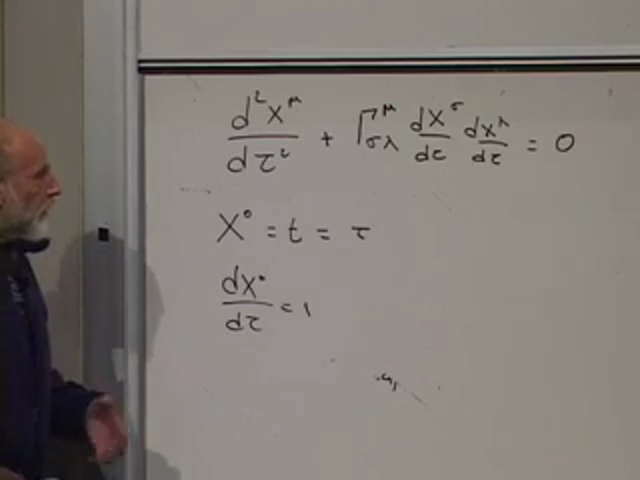
\includegraphics[width=0.84\textwidth]{lecture_08_figure_14.png}
  \caption{The slow-motion identification
  \(x^0=t\simeq\tau\) and \(dx^0/d\tau\simeq1\), displayed beside the
  full geodesic equation.}
  \lectureframe{01:18:45}
\end{figure}

In the product of two four-velocity components, the dominant term is
therefore the \(00\) term. For a spatial index \(i\),
\begin{equation}
  \frac{d^2x^i}{dt^2}
  \simeq
  -\Gamma^i{}_{00}.
  \label{eq:l08-acceleration-connection}
\end{equation}
The connection is not itself a tensor, but in this chosen weak-field
frame this component is the relativistic expression that reduces to the
Newtonian acceleration field.

\begin{figure}[tbp]
  \centering
  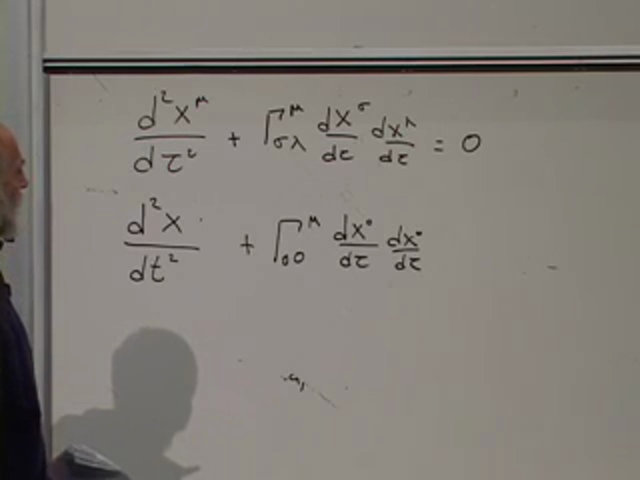
\includegraphics[width=0.86\textwidth]{lecture_08_figure_15.png}
  \caption{The spatial geodesic equation after retaining the dominant
  \(dx^0/d\tau\) factors. The remaining connection component is
  \(\Gamma^i{}_{00}\).}
  \lectureframe{01:21:45}
\end{figure}

\begin{classroomqa}
\audiencequestion{Why are both lower indices on the surviving
Christoffel symbol zero?
\lecturetimestamp{01:21:09--01:22:18}}
\lecturerresponse{Each lower index contracts with one component of the
four-velocity. The spatial components \(dx^i/d\tau\) are small, while
\(dx^0/d\tau\simeq1\). Keeping the leading term therefore selects
\(\Gamma^i{}_{00}\).}
\end{classroomqa}

\section{The Time--Time Metric Component as Potential}

Expand the relevant connection:
\begin{equation}
  \Gamma^i{}_{00}
  =
  \frac12 g^{i\rho}
  \left(
    2\partial_0g_{\rho0}
    -
    \partial_\rho g_{00}
  \right).
  \label{eq:l08-gamma-i00-exact}
\end{equation}
The derivatives of the Minkowski part vanish, so every derivative in
this expression is already first order in \(h_{\mu\nu}\). Replacing the
outside inverse metric by \(\eta^{\mu\nu}\) is therefore consistent:
including its \(O(h)\) correction would produce only \(O(h^2)\) terms.

The slowly varying source assumption makes the time derivatives
\(\partial_0g_{\rho0}\) negligible. Since
\(\eta^{ij}=-\delta^{ij}\), we obtain
\begin{equation}
  \Gamma^i{}_{00}
  \simeq
  \frac12\delta^{ij}\partial_jg_{00},
  \label{eq:l08-gamma-i00-static}
\end{equation}
and hence
\begin{equation}
  \boxed{
  \frac{d^2x^i}{dt^2}
  \simeq
  -\frac12\delta^{ij}\partial_jg_{00}.}
  \label{eq:l08-metric-acceleration}
\end{equation}

\begin{figure}[tbp]
  \centering
  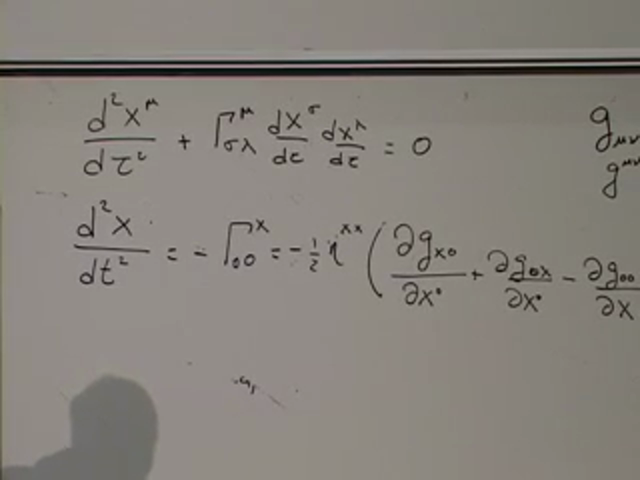
\includegraphics[width=0.92\textwidth]{lecture_08_figure_16.png}
  \caption{The weak-field expansion of
  \(\Gamma^i{}_{00}\). The connection contains two time derivatives of
  mixed metric components and one spatial derivative of \(g_{00}\).}
  \lectureframe{01:26:15}
\end{figure}

The live sign bookkeeping pauses several times here, and rightly so:
with signature \(+---\), losing one minus sign would turn attractive
gravity into repulsive gravity. Keeping the metric convention explicit
settles the result. Newtonian motion obeys
\begin{equation}
  \frac{d^2x^i}{dt^2}
  =
  -\delta^{ij}\partial_j\Phi.
  \label{eq:l08-newton-acceleration}
\end{equation}
Comparing Eqs.~\eqref{eq:l08-metric-acceleration} and
\eqref{eq:l08-newton-acceleration} gives
\begin{equation}
  \partial_i g_{00}=2\partial_i\Phi.
  \label{eq:l08-gradient-comparison}
\end{equation}

\begin{figure}[tbp]
  \centering
  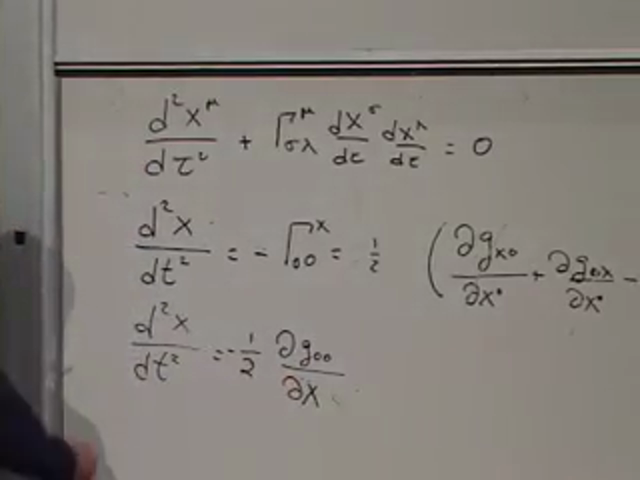
\includegraphics[width=0.86\textwidth]{lecture_08_figure_17.png}
  \caption{The board comparison between geodesic acceleration and the
  gradient of the Newtonian potential. The boxed relation isolates the
  spatial derivative of \(g_{00}\).}
  \lectureframe{01:28:00}
\end{figure}

Integration determines the relation only up to a constant:
\begin{equation}
  g_{00}=C+2\Phi.
  \label{eq:l08-g00-constant}
\end{equation}
Far from an isolated source, \(\Phi\to0\) and the metric approaches
Minkowski spacetime, so \(C=1\). Thus
\begin{equation}
  \boxed{g_{00}\simeq1+2\Phi}
  \qquad(c=1).
  \label{eq:l08-g00-potential}
\end{equation}
Restoring units gives \(g_{00}\simeq1+2\Phi/c^2\).

\begin{figure}[tbp]
  \centering
  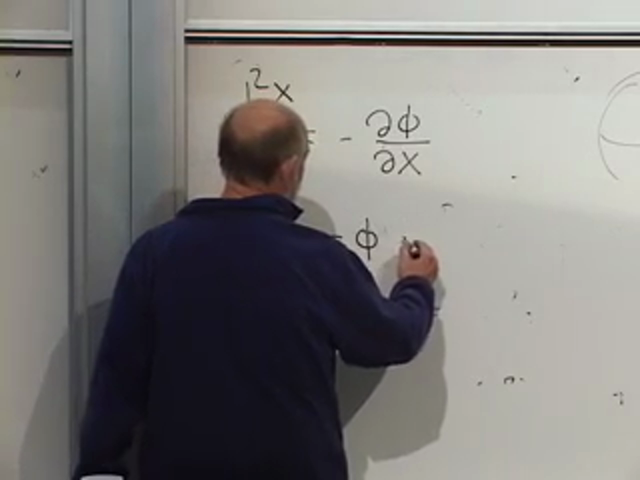
\includegraphics[width=0.78\textwidth]{lecture_08_figure_18.png}
  \caption{Newtonian acceleration above the integrated board relation
  between the time--time metric component and the potential. The
  additive constant is fixed by the asymptotically flat limit.}
  \lectureframe{01:31:00}
\end{figure}

\begin{classroomqa}
\audiencequestion{Why does the comparison determine a constant and a
factor of two rather than simply \(g_{00}=\Phi\)?
\lecturetimestamp{01:30:34--01:31:51}}
\lecturerresponse{The acceleration comparison equates gradients, so an
additive constant is invisible. The factor of two comes from the
\(\tfrac12\) in the Christoffel symbol. The boundary condition
\(g_{00}\to1\) where \(\Phi\to0\) fixes the constant.}
\end{classroomqa}

\section{Poisson's Equation and the Source}

Let \(\mathbf a(\mathbf x)\) be the Newtonian acceleration field. With
the convention used above,
\begin{equation}
  \mathbf a=-\boldsymbol{\nabla}\Phi.
  \label{eq:l08-acceleration-field}
\end{equation}
Gauss's law for Newtonian gravity is
\begin{equation}
  \boldsymbol{\nabla}\cdot\mathbf a
  =
  -4\pi G\rho,
  \label{eq:l08-newton-gauss}
\end{equation}
so the potential obeys Poisson's equation:
\begin{equation}
  \boxed{\nabla^2\Phi=4\pi G\rho,}
  \qquad
  \nabla^2
  =
  \partial_x^2+\partial_y^2+\partial_z^2.
  \label{eq:l08-poisson}
\end{equation}

\begin{figure}[tbp]
  \centering
  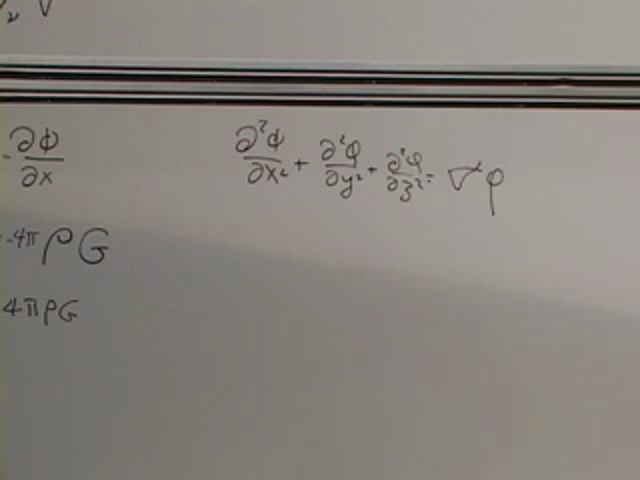
\includegraphics[width=0.84\textwidth]{lecture_08_figure_19.png}
  \caption{The Newtonian chain on the board: acceleration as a
  potential gradient, the divergence law, and Poisson's equation with
  its three-dimensional Laplacian.}
  \lectureframe{01:35:30}
\end{figure}

In units \(c=1\), rest-mass density is the leading contribution to
energy density. In the slow-moving frame,
\begin{equation}
  T_{00}\simeq T^{00}\simeq\rho.
  \label{eq:l08-density-t00}
\end{equation}
Poisson's equation can therefore be written
\begin{equation}
  \nabla^2\Phi
  =
  4\pi G T_{00}.
  \label{eq:l08-poisson-t00}
\end{equation}
Using \(g_{00}=1+2\Phi\), the constant disappears under the Laplacian:
\begin{equation}
  \boxed{\nabla^2g_{00}=8\pi G T_{00}.}
  \label{eq:l08-weak-field-component-equation}
\end{equation}
We have learned that a metric component is controlled by an
energy--momentum component. This is already the seed of the
gravitational field equation.

\begin{figure}[tbp]
  \centering
  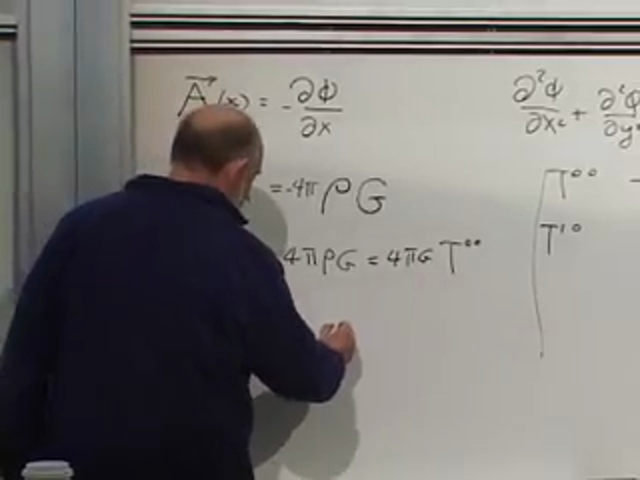
\includegraphics[width=0.9\textwidth]{lecture_08_figure_20.png}
  \caption{Poisson's equation rewritten with the \(00\) entry of the
  stress--energy tensor, followed by the weak-field equation for
  \(g_{00}\).}
  \lectureframe{01:37:45}
\end{figure}

\section{From One Component to a Tensor Equation}

Equation~\eqref{eq:l08-weak-field-component-equation} is useful but not
yet generally covariant. It was derived in a special frame where
velocities are small, the field is weak, and time dependence is slow.
The right-hand side is one component of a tensor, while the left-hand
side is written as a three-dimensional Laplacian of one selected metric
component. A fundamental equation must instead equate complete tensors.

\begin{classroomqa}
\audiencequestion{What is wrong with
\(\nabla^2g_{00}=8\pi G T_{00}\) if it gives the correct Newtonian
limit?
\lecturetimestamp{01:38:08--01:39:40}}
\lecturerresponse{Nothing is wrong with it inside the approximation in
which it was derived. It is incomplete because it is not manifestly a
tensor equation and singles out one frame and one component. We seek a
covariant equation whose \(00\) component reduces to it in the
Newtonian regime.}
\end{classroomqa}

Call the desired geometric tensor \(G_{\mu\nu}\). It must
\begin{enumerate}
  \item have two indices, like \(T_{\mu\nu}\);
  \item be built from the metric;
  \item contain the second-derivative curvature structure; and
  \item reproduce Eq.~\eqref{eq:l08-weak-field-component-equation} in
  the Newtonian limit.
\end{enumerate}
The target equation is
\begin{equation}
  G_{\mu\nu}=8\pi G T_{\mu\nu}.
  \label{eq:l08-target-field-equation}
\end{equation}

\begin{figure}[tbp]
  \centering
  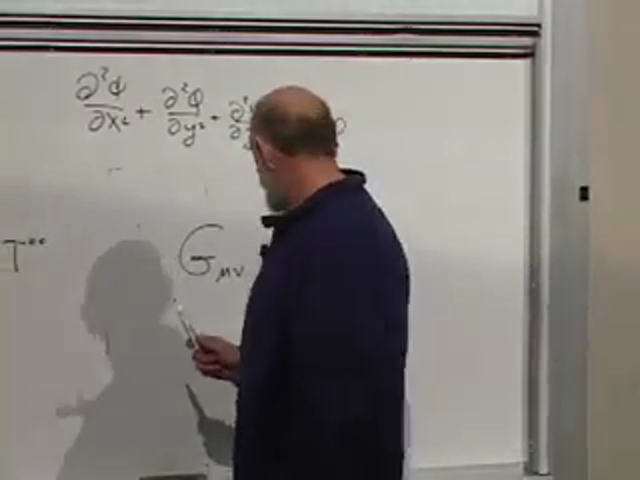
\includegraphics[width=0.9\textwidth]{lecture_08_figure_21.png}
  \caption{The weak-field component equation beside the proposed
  covariant form \(G_{\mu\nu}=8\pi G T_{\mu\nu}\). The unknown left-hand
  side must be made entirely from the metric and curvature.}
  \lectureframe{01:40:30}
\end{figure}

The available symmetric two-index curvature tensors are
\(R_{\mu\nu}\) and \(g_{\mu\nu}R\). Under the assumptions being used in
the lecture, the candidate is therefore
\begin{equation}
  A R_{\mu\nu}
  +
  B g_{\mu\nu}R
  =
  8\pi G T_{\mu\nu},
  \label{eq:l08-ab-ansatz}
\end{equation}
where \(A\) and \(B\) are numerical coefficients. An overall
normalization can be absorbed into Newton's constant; the nontrivial
question is the relative coefficient.

\begin{figure}[tbp]
  \centering
  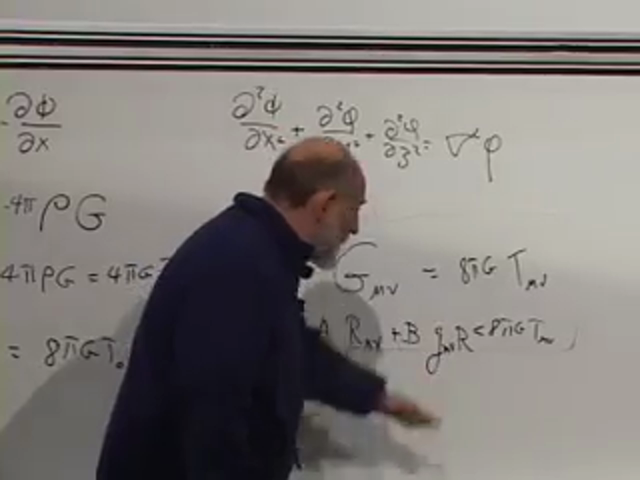
\includegraphics[width=0.92\textwidth]{lecture_08_figure_22.png}
  \caption{The final board ansatz: a linear combination of the Ricci
  tensor and \(g_{\mu\nu}R\) is matched to the stress--energy tensor.}
  \lectureframe{01:43:30}
\end{figure}

The lecture stops before deriving the coefficients, but it reveals the
destination:
\begin{equation}
  G_{\mu\nu}
  =
  R_{\mu\nu}
  -
  \frac12g_{\mu\nu}R.
  \label{eq:l08-einstein-tensor-preview}
\end{equation}
Why precisely this combination is selected, how its divergence relates
to local energy--momentum conservation, and how its normalization
recovers Newtonian gravity are the next steps. For now the logic is
already visible:
\[
  \begin{aligned}
    \text{geodesics}
    &\longrightarrow g_{00}\simeq1+2\Phi\\
    &\longrightarrow \nabla^2\Phi=4\pi G\rho\\
    &\longrightarrow G_{\mu\nu}=8\pi G T_{\mu\nu}.
  \end{aligned}
\]

\begin{classroomqa}
\audiencequestion{Are the coefficients difficult numbers?
\lecturetimestamp{01:45:13--01:45:33}}
\lecturerresponse{No. With the Ricci term normalized to one, the second
coefficient is \(-\tfrac12\). The simplicity of the numbers is not the
reason for the combination; the geometric conservation identity is.}
\end{classroomqa}

\section{What We Have Established}

The operator notation
\(\nabla_\mu=\partial_\mu+\Gamma_\mu\) turns the geometric experiment of
parallel transport into a calculation. A difference of differences
around an infinitesimal loop is a commutator of covariant derivatives,
and the resulting operator is the Riemann tensor. Its pair
antisymmetries, pair exchange, and Bianchi identity determine its
component structure; its mixed contractions produce the Ricci tensor
and scalar curvature.

The same lecture then places the geometry under physical pressure. A
slowly moving particle in a weak, nearly static field follows a geodesic
whose spatial acceleration is
\(-\Gamma^i{}_{00}\). With signature \(+---\), this identifies
\(g_{00}\simeq1+2\Phi\). Newtonian Poisson theory then becomes the
component relation
\(\nabla^2g_{00}=8\pi G T_{00}\).

That component equation cannot be the final theory because it belongs
to one approximation and one frame. The lecture therefore ends with a
sharply posed reconstruction problem: find a symmetric two-index
curvature tensor whose Newtonian limit is the component equation and
whose covariant form can stand opposite \(T_{\mu\nu}\). The only
available combination is poised to become the Einstein tensor.
